\documentclass[aspectratio=169]{beamer}

\usetheme{default}
\usecolortheme{dolphin}
\setbeamertemplate{navigation symbols}{}
\setbeamertemplate{footline}[frame number]
\setbeamerfont{frametitle}{size=\large}
\setbeamercolor{frametitle}{fg=black}

\usepackage[T1]{fontenc}
\usepackage[utf8]{inputenc}
\usepackage{graphicx}
\usepackage{booktabs}
\usepackage{amsmath}
\usepackage{bm}

\title{Görsel-Ataletsel Odometri Sapmasının Kendi Kendine Öğrenen\\
Havadan Coğrafi Konumlandırma ile Sınırlandırılması}
\subtitle{GNSS'siz İHA seyrüseferi, yalnızca CPU üzerinde}
\author{Nijat Abbasov}
\date{\today}

\begin{document}

\begin{frame}
\titlepage
\end{frame}

\begin{frame}{İki kestirici, birbirinin zıddı iki zayıflık}
\begin{columns}[T]
\begin{column}{0.5\textwidth}
\textbf{VIO} --- pürüzsüz, ama hatası sınırsız büyür\\
{\small 3,6 km'de 700 m $=$ kat edilen mesafenin \%19'u}

\vspace{0.9em}
\textbf{Coğrafi konumlandırma} --- mutlak, hiç sapmaz\\
{\small ancak eşleşmelerin yalnızca \%36'sı doğru}

\vspace{1.3em}
\textbf{İkisini birleştir.}\\
{\small VIO yörüngenin şeklini verir.\\
Coğrafi konumlandırma ölçeği ve mutlak konumu verir.}

\vspace{1.3em}
{\small MUN-FRL \texttt{bell412\_dataset4}\\
3,6 km, Ottawa Uluslararası Havalimanı\\
Yalnızca CPU --- hava aracında GPU yok}
\end{column}
\begin{column}{0.5\textwidth}
\centering
\vspace{1.5em}
\begin{tabular}{@{}lcc@{}}
\toprule
 & OpenVINS & Birleşik \\
\midrule
Gerçek zamanlı RMSE & 489\,m & \textbf{248\,m} \\
En iyi koşu & 464\,m & \textbf{198\,m} \\
\bottomrule
\end{tabular}

\vspace{2em}
{\large $-\%49$}\\[0.2em]
{\small üç koşunun ortalaması}

\vspace{1em}
{\large $-\%57$}\\[0.2em]
{\small en iyi koşu}
\end{column}
\end{columns}
\end{frame}

\begin{frame}{CAEVL --- eşleştirilmiş veri gerektirmeyen konumlandırma}
\begin{columns}[T]
\begin{column}{0.48\textwidth}
\textbf{Alan farkı:} şimdi çekilen fotoğraf ile aylar önceki uydu görüntüsü.

\vspace{0.7em}
\textbf{Çözüm:} görünümü tamamen at --- her iki taraf da \textbf{Canny kenar
haritasına} dönüştürülür.

\vspace{1em}
\textbf{Eğitim yalnızca referans görüntüyle:}
\begin{enumerate}
\item Otokodlayıcı $\rightarrow$ 1024 boyutlu betimleyici\\{\small $+$ DINOv2 algısal kaybı}
\item Temiz/bozulmuş çiftler üzerinde VICReg\\{\small negatif örnek ve eşleştirilmiş İHA verisi gerekmez}
\end{enumerate}

\vspace{0.9em}
$\Rightarrow$ yeni bir araziye geçmek için \textbf{yalnızca uydu görüntüsü} yeter
\end{column}
\begin{column}{0.5\textwidth}
\centering
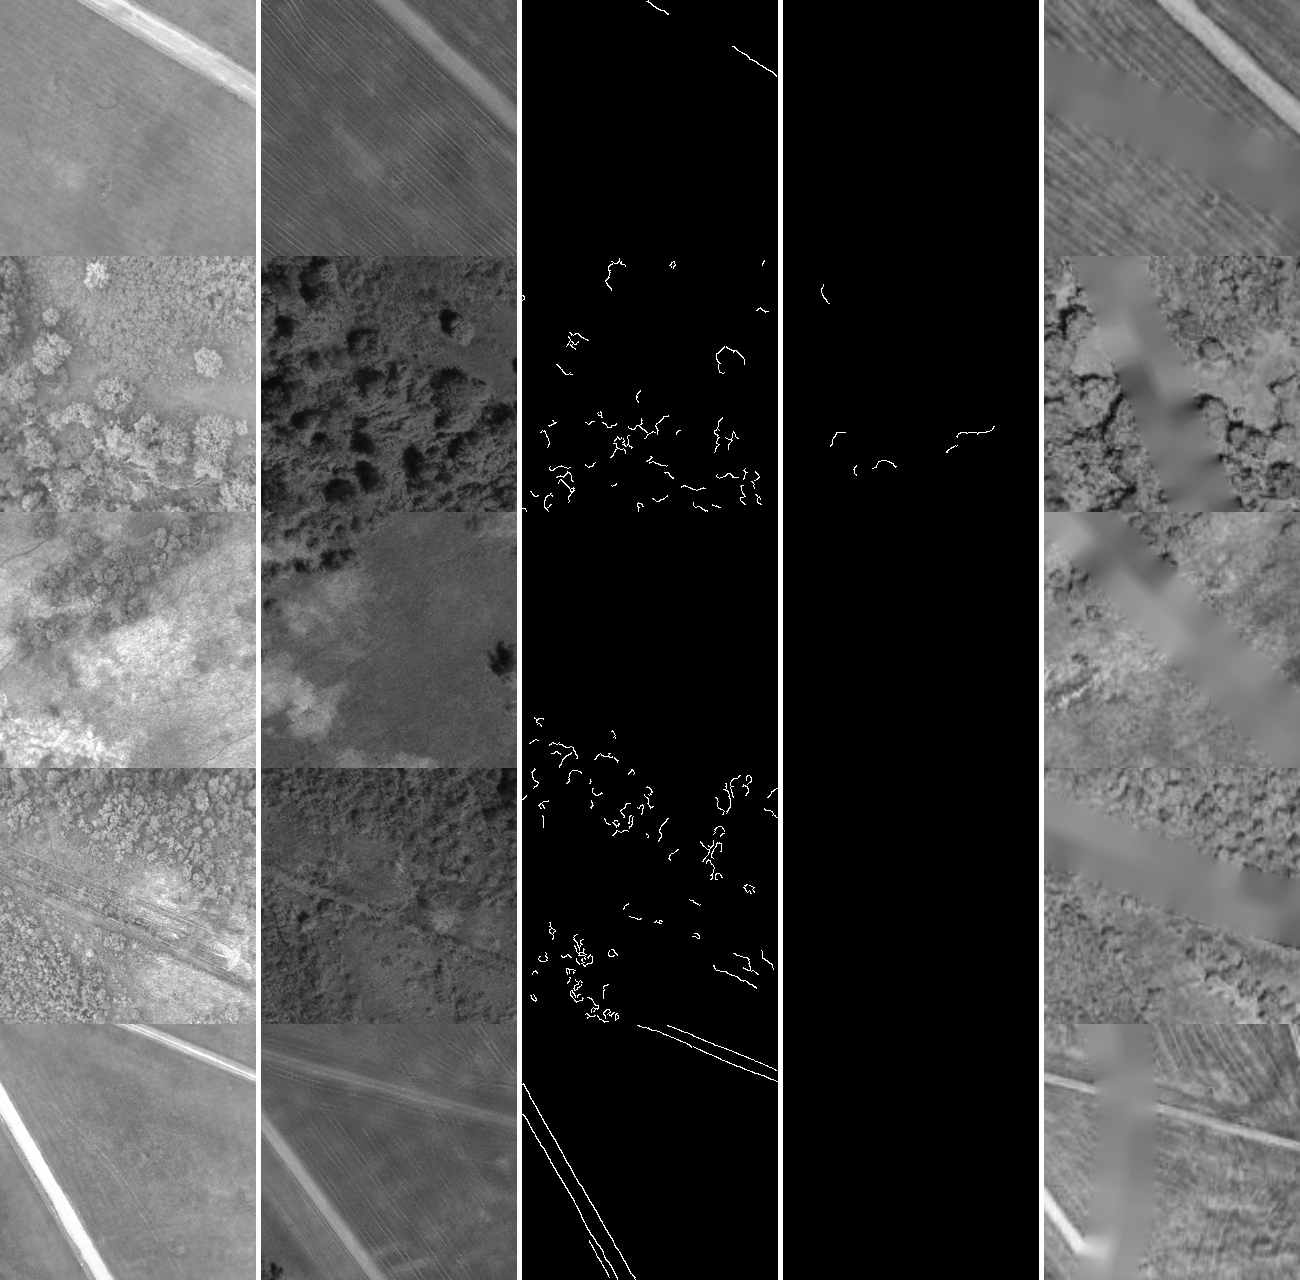
\includegraphics[width=0.8\linewidth]{figures/esri_vs_munfrl.png}

\vspace{0.7em}
\begin{tabular}{@{}lc@{}}
\toprule
ViLD tekrar üretimi & R@1 \\
\midrule
Makale & \%49,68 \\
Bizim & \%48,14 \\
\quad $+$ algısal kayıp & \textbf{\%52,88} \\
\bottomrule
\end{tabular}
\end{column}
\end{columns}
\end{frame}

\begin{frame}{OpenVINS --- ve veri kümesi sorunu}
\begin{columns}[T]
\begin{column}{0.44\textwidth}
Bir kamera $+$ bir IMU. Daha önce geçtiği yerleri tanımaz, bu yüzden hata
yalnızca birikir.

\vspace{0.6em}
Kalkış noktasından başlayarak \textbf{14,7 m} sapmayla başlar, 3,6 km sonunda
\textbf{700 m} sapar.

\vspace{0.6em}
Yörüngenin \emph{şekli} doğru, ancak \textbf{fazla küçük} çıkıyor --- sanki tüm
uçuş küçültülmüş gibi. Geri esnetmek hatanın çoğunu düzeltiyor.

\vspace{0.8em}
\textbf{Neden kullanılabilir veri kümesi bu kadar az?}\\[0.3em]
{\small Kamera takibi \textbf{alçak} uçmak ister\\
{\scriptsize kareler arasında nesneler daha çok hareket eder}\\[0.2em]
Harita eşleştirme \textbf{yüksek} uçmak ister\\
{\scriptsize her fotoğraf daha geniş bir alanı kapsar}}
\end{column}
\begin{column}{0.56\textwidth}
\centering
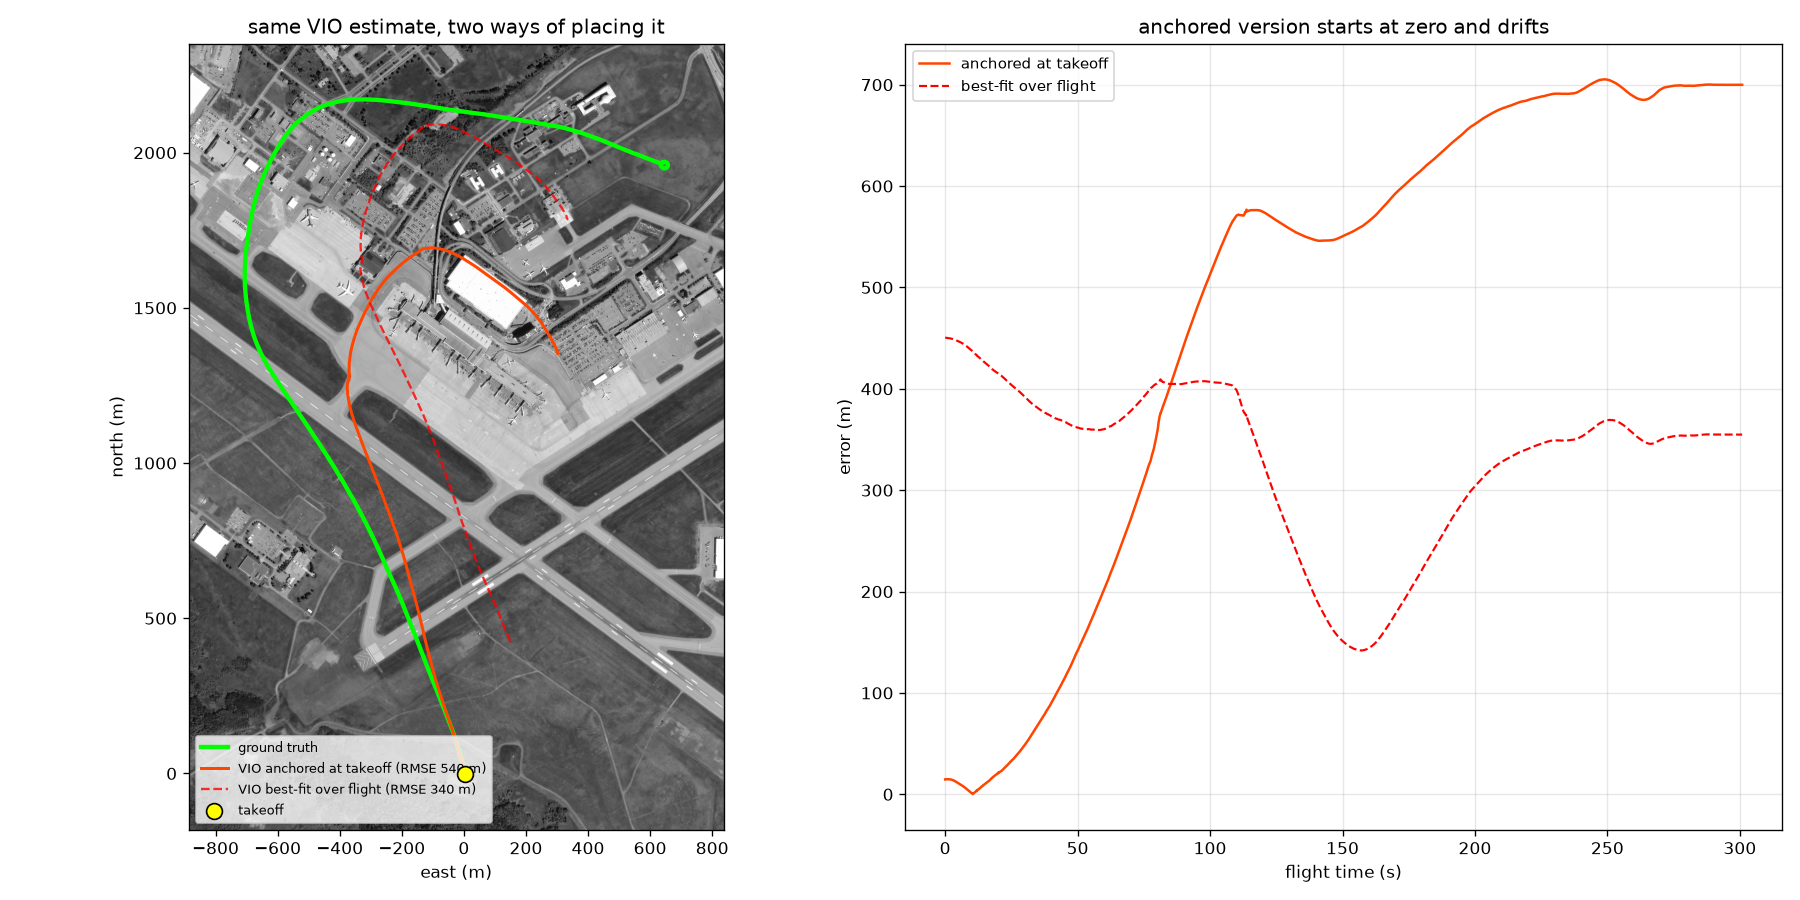
\includegraphics[width=\linewidth]{figures/vio_anchoring_dataset4.png}

\vspace{0.5em}
{\small
\begin{tabular}{@{}llc@{}}
\toprule
Veri kümesi & İrtifa & IMU \\
\midrule
VPAIR & 300\,m & yok \\
AerialVL & --- & yok \\
SatLoc & 100--300\,m & yayınlanmamış \\
Zurich MAV & 5--15\,m & çok alçak \\
\textbf{MUN-FRL} & \textbf{25--170\,m} & \textbf{var} \\
\bottomrule
\end{tabular}}
\end{column}
\end{columns}
\end{frame}

\begin{frame}{Hangi eşleşmelere güvenebiliriz?}
\begin{columns}[T]
\begin{column}{0.4\textwidth}
Eşleşmelerin yalnızca \textbf{\%36'sı} doğru --- üstelik ağın kendi güven skoru
\emph{yanlışken daha yüksek}:

\vspace{0.5em}
\centering
\begin{tabular}{@{}lcc@{}}
\toprule
güven & doğru & yanlış \\
\midrule
uçuş 1 & 0,9429 & \textbf{0,9493} \\
uçuş 2 & 0,9447 & \textbf{0,9598} \\
\bottomrule
\end{tabular}

\vspace{1em}
\raggedright
\textbf{Bu yüzden güven skorunu tamamen yok sayıyoruz.}

\vspace{0.7em}
Bunun yerine: aracın aralarında ne kadar yol aldığı hesaba katıldığında
\textbf{birbiriyle tutarlı olan} eşleşmeleri tutuyoruz.

\vspace{0.5em}
{\small Yanlış eşleşmeler rastgele yerlere düşer --- ikisinin aynı yerde
buluşması \%0,5'lik bir tesadüf. Doğru olanlar ise kendiliğinden uyuşur.}
\end{column}
\begin{column}{0.58\textwidth}
\centering
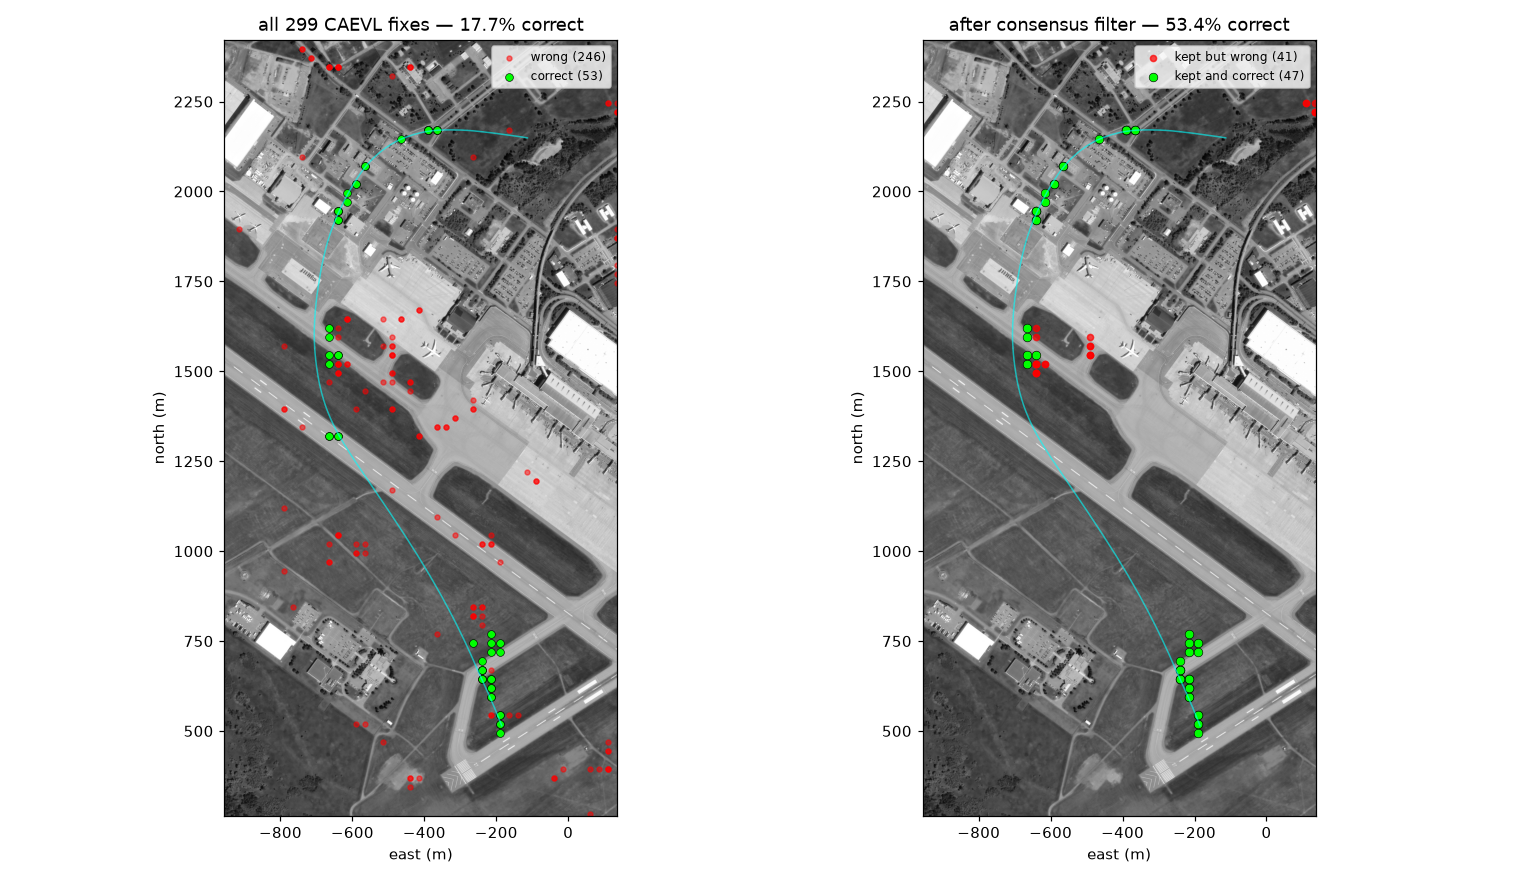
\includegraphics[width=\linewidth]{figures/consensus_filter.png}

\vspace{0.4em}
\begin{tabular}{@{}lcc@{}}
\toprule
 & önce & sonra \\
\midrule
eşleşme & 299 & 101 \\
doğruluk & \%17,7 & \textbf{\%99,0} \\
korunan doğru & 107 & 100 \textbf{(\%93)} \\
\bottomrule
\end{tabular}
\end{column}
\end{columns}
\end{frame}

\begin{frame}{Nedensel (gerçek zamanlı) birleştirme}
\centering
$\hat{\bm{p}}_k = s\,\bm{R}(\theta)\,\bm{p}^{\text{vio}}_k + \bm{t}$
\quad --- çevrim içi, \textbf{yalnızca geçmiş eşleşmelerden} kestirilir

\vspace{1.2em}
\begin{columns}[T]
\begin{column}{0.47\textwidth}
\raggedright
\textbf{Her yeni eşleşmede}
\begin{enumerate}
\item eşleşme bir tampona alınır
\item \emph{geçmişe dönük} pencere tutarlılık için taranır
\item hayatta kalanlar biriktirilir
\item $(s,\theta,\bm{t})$ tüm kabul edilmiş geçmişe yeniden oturtulur
\end{enumerate}

\vspace{0.9em}
\textbf{Devir alınana kadar:} bilinen kalkış noktasından VIO ile ölü hesap\\
{\small $\Rightarrow$ \emph{her} an bir konum çıktısı verilir}
\end{column}
\begin{column}{0.47\textwidth}
\raggedright
\textbf{Neden $s$ ve $\theta$ kestiriliyor?}\\[0.3em]
{\small Sistem kuzeyin nerede olduğunu bilmeden başlar ve VIO yörüngesi fazla
küçük çıkar --- ikisi de eşleşmelerden öğrenilmelidir.}

\vspace{1.2em}
\textbf{Kalman filtresi denendi ve kaybetti: 422 m'ye karşı 347 m}\\[0.3em]
{\small Ölçek hatası \emph{doğrusal} büyür, süreç gürültüsü ise $\sqrt{\cdot}$
ile. Filtre aşırı özgüvenli hâle gelir ve doğru eşleşmeleri eler --- en çok
yanıldığı anda en emin olur.}
\end{column}
\end{columns}
\end{frame}

\begin{frame}{Sonuç --- gerçek zamanlı, tüm uçuş}
\centering
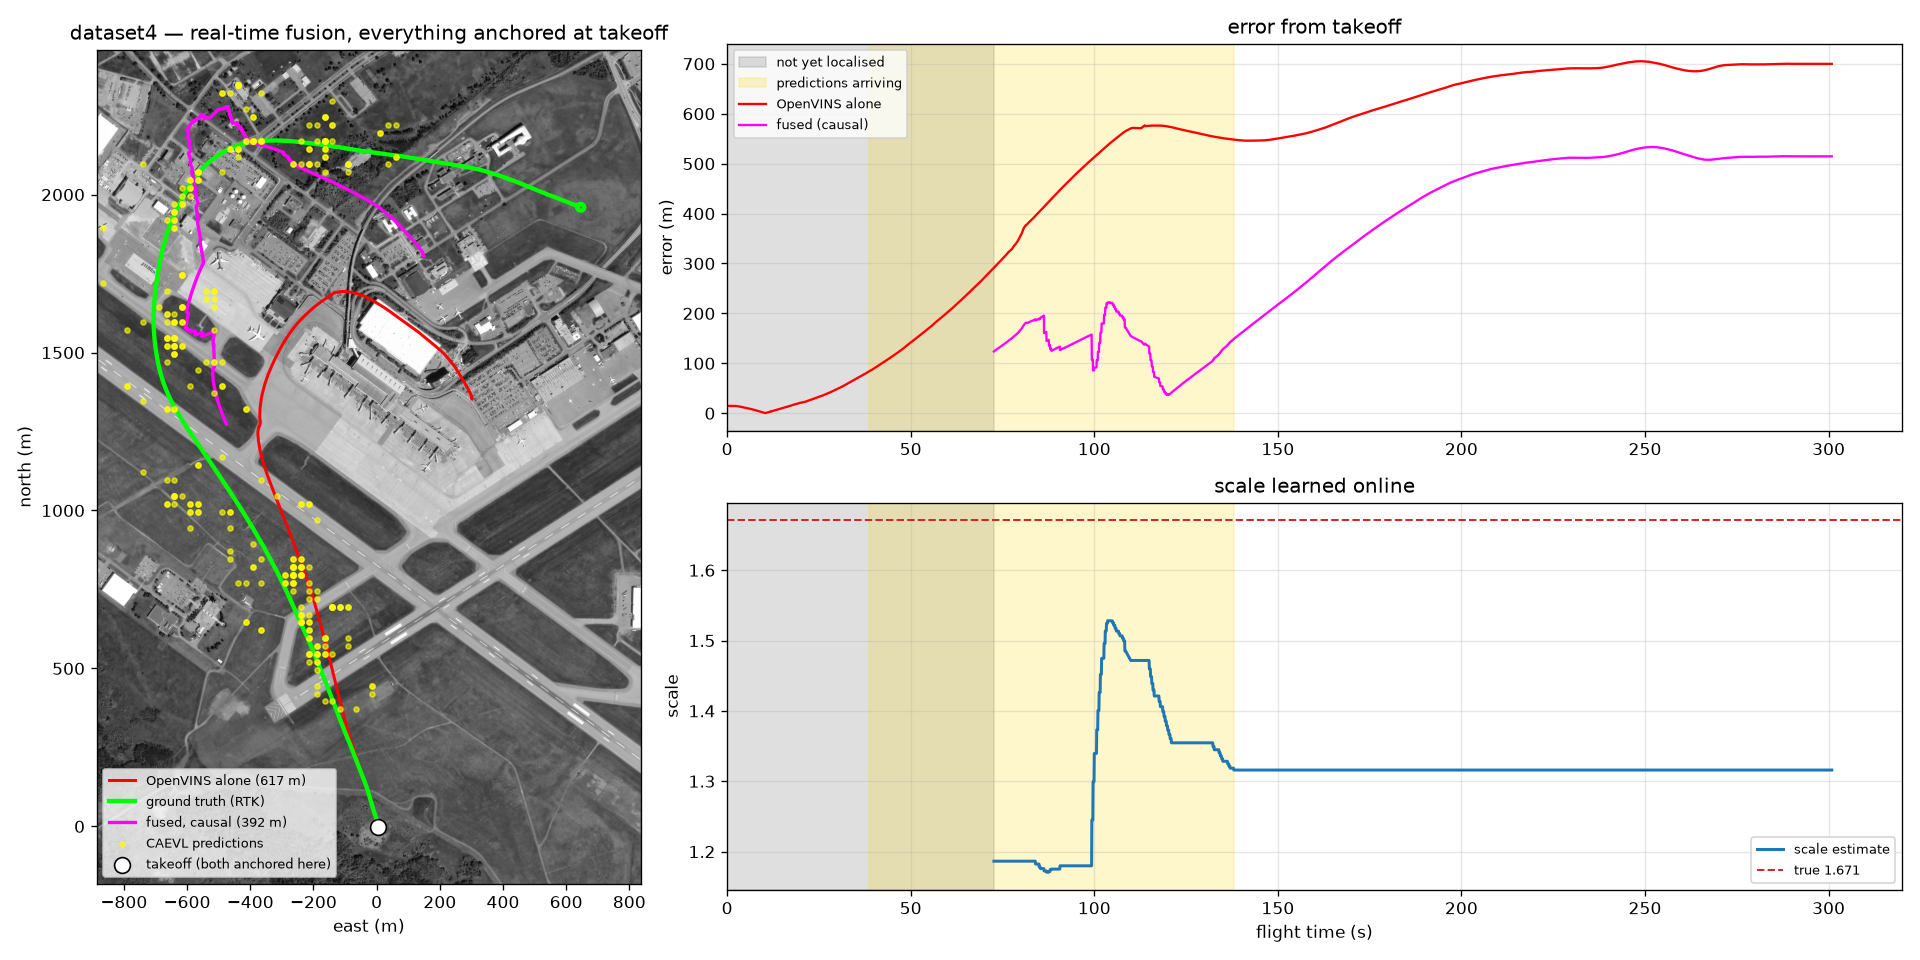
\includegraphics[width=0.9\linewidth]{figures/FINAL_causal_dataset4.png}

\vspace{-0.3em}
{\small Kırmızı: yalnızca OpenVINS. Yeşil: RTK gerçek referans. Macenta:
birleşik. Gri: devir alınmadan önce ölü hesap ($t{+}73$\,s).
\quad\textbf{464\,m $\rightarrow$ 198\,m}}
\end{frame}

\begin{frame}{Özet --- doğruluk}
\centering
\begin{tabular}{@{}lccc@{}}
\toprule
 & Yalnızca OpenVINS & \textbf{$+$ Coğrafi kon.} & İyileşme \\
\midrule
Konum hatası (RMSE) & $489 \pm 44$\,m & $\bm{248 \pm 86}$\,\textbf{m} & $-\%49$ \\
\quad en iyi koşu   & 463,8\,m & \textbf{198,2\,m} & $-\%57$ \\
Uçuş boyunca sapma  & $\%17,7 \pm 1,5$ & $\bm{\%10,1 \pm 3,6}$ & $-\%43$ \\
\midrule
Yönelim hatası & \multicolumn{3}{c}{\emph{ölçülemiyor --- bu veri kümesinde referans yönelim yok}} \\
\bottomrule
\end{tabular}

\vspace{1.2em}
{\small Sapma, son konum hatasının kat edilen mesafeye oranıdır:
\textbf{3,6 km sonunda araç gerçekte olduğu yerden bu mesafenin \%10'u kadar
uzakta}, \%18 yerine.}

\vspace{0.8em}
{\small Aynı girdilerle yapılan üç OpenVINS koşusunun ortalaması. Her iki yörünge
de bilinen kalkış noktasından başlar; sistem yalnızca o anda mevcut olan bilgiyi
kullanır.}
\end{frame}

\begin{frame}{Özet --- hava aracında çalışabilir mi?}
\centering
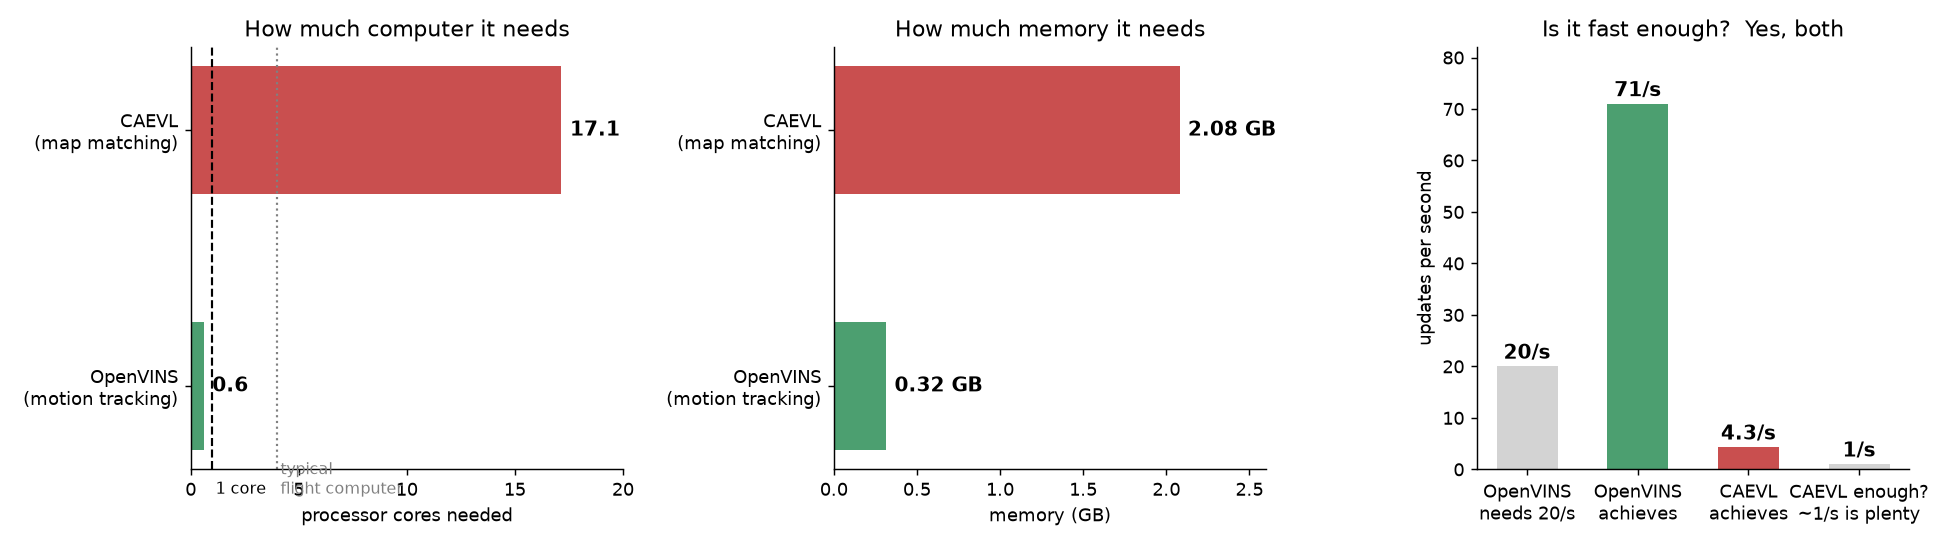
\includegraphics[width=\linewidth]{figures/compute_cost.png}

\vspace{0.6em}
\begin{columns}
\begin{column}{0.46\textwidth}
\textbf{Hareket takibi} ucuz\\
{\small bir çekirdekten az, 0,3 GB ve kameranın ihtiyacından 3,5 kat hızlı}
\end{column}
\begin{column}{0.5\textwidth}
\textbf{Harita eşleştirme} pahalı olan kısım\\
{\small burada 17 çekirdek. Tek çekirdekte 4 saniyede bir konum verirdi --- yine
de yeterli, çünkü mutlak konuma yalnızca ara sıra ihtiyaç var.}
\end{column}
\end{columns}
\end{frame}

\begin{frame}{Kısıtlar ve sonraki adımlar}
\begin{columns}[T]
\begin{column}{0.5\textwidth}
\textbf{Sınırlayıcı etken doğruluk değil, erişilebilirlik}
\begin{itemize}
\item 100 m'lik bir harita karosu için $\sim$66 m irtifa gerekir\\
      {\small bu uçuşun yalnızca \textbf{\%34'ü} bu koşulu sağlıyor}
\item Bunun altında: \%1--5 doğruluk\\
      {\small denendi --- eklemek sonucu \emph{kötüleştirdi}: 347 $\rightarrow$ 527\,m}
\item Daha küçük karolar betimleyicileri çökertiyor\\
      {\small çiftlerin \%2,21'i $>0,99$ benzer, 100 m'de \%0,31}
\item İrtifa ve başlangıç yönü hâlâ gerçek referanstan\\
      {\small sahada: altimetre $+$ manyetometre}
\end{itemize}
\end{column}
\begin{column}{0.48\textwidth}
\textbf{Sonraki adımlar}
\begin{enumerate}
\item \textbf{Sorgu tarafında ölçek normalizasyonu}\\
      {\small en düşük çalışma irtifasında tek bir veri tabanı; sorguları ona indir}
\item \textbf{Doğru boyutta karolarla yeniden eğitim}\\
      {\small 1438 m'lik alanı kapsayan karolarla eğitildi, 100 m'de kullanılıyor
      --- 14 kat uyumsuzluk}
\item \textbf{VIO yörüngesinin neden küçük çıktığını bul}\\
      {\small koşular arası farkın da kaynağı: aynı girdiyle 540'a karşı 464\,m}
\end{enumerate}

\vspace{1.2em}
\centering
\footnotesize
\texttt{github.com/NijatAbbasov06/}\\
\texttt{uav-geolocalization}
\end{column}
\end{columns}
\end{frame}

\end{document}
